%%%%%%%%%%%%%%%%%%%%%%%%%%%%%%%%%%%%%%%%%
% fphw Assignment
% LaTeX Template
% Version 1.0 (27/04/2019)
%
% This template originates from:
% https://www.LaTeXTemplates.com
%
% Authors:
% Class by Felipe Portales-Oliva (f.portales.oliva@gmail.com) with template
% content and modifications by Vel (vel@LaTeXTemplates.com)
%
% Template (this file) License:
% CC BY-NC-SA 3.0 (http://creativecommons.org/licenses/by-nc-sa/3.0/)
%
%%%%%%%%%%%%%%%%%%%%%%%%%%%%%%%%%%%%%%%%%

%----------------------------------------------------------------------------------------
%	PACKAGES AND OTHER DOCUMENT CONFIGURATIONS
%----------------------------------------------------------------------------------------

\documentclass[
    12pt, % Default font size, values between 10pt-12pt are allowed
%letterpaper, % Uncomment for US letter paper size
%spanish, % Uncomment for Spanish
]{../fphw}

% Template-specific packages
\usepackage[utf8]{inputenc} % Required for inputting international characters
\usepackage[T1]{fontenc} % Output font encoding for international characters
\usepackage{mathpazo} % Use the Palatino font

\usepackage{graphicx} % Required for including images

\usepackage{booktabs} % Required for better horizontal rules in tables

\usepackage{listings} % Required for insertion of code

\usepackage{enumerate} % To modify the enumerate environment
\usepackage{textcomp}
\usepackage{amsmath}
\usepackage{subcaption}
\usepackage[justification=centering]{caption}
\usepackage{float}
\usepackage{xcolor}
\usepackage{polski}
\usepackage[polish]{babel}
\usepackage{csvsimple}
\usepackage{mathtools}
\usepackage{ulem}
\usepackage{hyperref}
\usepackage{makecell}
\usepackage{multirow}
\renewcommand{\cellalign}{cl}
\usepackage[ddmmyyyy]{datetime}
\renewcommand{\dateseparator}{.}

\definecolor{codegreen}{rgb}{0,0.6,0}
\definecolor{codegray}{rgb}{0.5,0.5,0.5}
\definecolor{codepurple}{rgb}{0.58,0,0.82}
\definecolor{backcolour}{rgb}{0.95,0.95,0.92}

\lstdefinestyle{mystyle}{
    backgroundcolor=\color{backcolour},
    commentstyle=\color{codegreen},
    keywordstyle=\color{magenta},
    numberstyle=\tiny\color{codegray},
    stringstyle=\color{codepurple},
    basicstyle=\ttfamily\footnotesize,
    breakatwhitespace=false,
    breakatwhitespace=false,
    breaklines=true,
    captionpos=b,
    keepspaces=true,
    numbers=left,
    numbersep=5pt,
    showspaces=false,
    showstringspaces=false,
    showtabs=false,
    tabsize=2
}

\lstset{style=mystyle}

\renewcommand{\lstlistlistingname}{Spis listingów}
%----------------------------------------------------------------------------------------
%	ASSIGNMENT INFORMATION
%----------------------------------------------------------------------------------------

\title{Projekt 1} % Assignment title

\author{inż.Monika Nawój} % Student name

\date{\today} % Due date

\institute{Politechnika Warszawska \\ Wydział Elektroniki i Technik Informacyjnych} % Institute or school name

\class{Zarządzanie i harmonogramowanie procesów} % Course or class name

\professor{mgr inż. Przemysław Kacprzak} % Professor or teacher in charge of the assignment

%----------------------------------------------------------------------------------------

\begin{document}

\maketitle % Output the assignment title, created automatically using the information in the custom commands above

%----------------------------------------------------------------------------------------
%	ASSIGNMENT CONTENT
%----------------------------------------------------------------------------------------

\section{Treść projektu}
O ile nie jest powiedziane inaczej, to jako rozwiązanie należy przesłać: model matematyczny problemu, pliki z modelem i danymi, uzyskane wyniki z
interpretacją. \\
Zadania do wykonania:
\begin{enumerate}
    \item Odpowiedzieć na pytanie, jak można zmiejszć liczbę zmiennych wykorzystywanych w zadaniu opisanym w podsekcji 3.2.
    \item Znaleźć najkrótszy czas wykonania przedsięwzięcia (dane są podane poniżej) - korzystając z grafu w postaci krawędziowej
    \item Zapisać i rozwiązać dla podanych danych problem stworzenia harmonogramu o minimalnym czasie wykonania, jako zadanie programowania
          liniowego. Podać uzyskany harmonogram.
    \item Wprowadzamy drobną modyfikację w tym zadaniu planowania. Zadania można skrócić poprzez przydział dodatkowych środków.
          Przydzielając dodatkowe \(\alpha_i\) środków skracam czas wykonania zadania \(i\) o 1
          dzień. Każde zadanie ma minimalny czas wykonywania zadania \(t^{min}\),
          poniżej którego się nie da skrócić. Rozwiązując to zadanie, uzyskamy
          minimalny czas realizacji przedsięwzięcia, przy określonym budżecie,
          czy w uzyskanym rozwiązaniu (w ogólnym przypadku) jest wykorzystywany minimalny budżet. W jaki sposób dobieramy zadania do skrócenia (w ogólnym przypadku)?
    \item Podobnie jak w poprzednim punkcie istnieje możliwość skracania czasów zadań. Dodatkowym ograniczeniem jest to, ze liczba skróconych
          zadań nie nie może przekroczyć NS. Czy zmienia sie warunki doboru zadań do skrócenia?
    \item Weźmy warunki z punktu 2 (tzn. bez mozliwości skracania zadań).
          Wprowadzamy drugi typ relacji poprzedzania: zadanie B nie może zakończyć sie przed zakończeniem zadania A. Zapisać i rozwiązać dla
          podanych danych zadanie w którym występują oba typy relacji poprzedzania.
\end{enumerate}
\subsection{Dane}
\begin{table}[H]
    \centering
    \begin{tabular} {| c | c | c | c | c |}
        \hline
        Zadanie & \(t\) & poprzedniki & \(\alpha\) & \(t^{min}\) \\
        \hline
        A       & 14    &             & 70         & 8           \\
        \hline
        B       & 8     & G           & 5          & 3           \\
        \hline
        C       & 14    & A           & 1          & 1           \\
        \hline
        D       & 8     & I           & 50         & 3           \\
        \hline
        E       & 5     &             & 90         & 5           \\
        \hline
        F       & 7     & B,H         & 80         & 3           \\
        \hline
        G       & 15    & A,E         & 75         & 6           \\
        \hline
        H       & 5     & D           & 100        & 1           \\
        \hline
        I       & 10    & E           & 50         & 6           \\
        \hline
        J       & 9     & G,I         & 20         & 5           \\
        \hline
    \end{tabular}
    \caption{Dane do projektu przedtawione w formie tabeli.}
    \label{tab:dane}
\end{table}
W punkcie 2 i 3 dostępne są środki do skracania zadań: 200. \\
W punkcie 3 NS = 2. \\
Dodatkowa relacja poprzedzania: \\
\begin{table}[H]
    \centering
    \begin{tabular}{| c | c |}
        \hline
        Zadanie poprzedzające & Następnik \\
        \hline
        C & B \\
        \hline
        D & G \\
        \hline
    \end{tabular}
    \caption{Dodatkowe relacje przedstawione w formie tabeli.}
    \label{tab:dod_rel}  
\end{table}
\newpage
\section{Rozwiązanie}
\subsection{Zmniejszenie liczby zmiennych wykorzystywanych w zadaniu opisanym w podsekcji 3.2}
Możliwe jest zmniejszenie liczby zmiennych wykorzystywanych w wyżej wymienionym
zadaniu przy wykorzystaniu metody ścieżki krytycznej (CPM).
Możemy się pozbyć się zmniennych związanych z momentem rozpoczęcia oraz zakończenia
wykonywania zadania \(j\) \((t^p_j, t^k_j)\) jeżeli przedstawimy porządek wykonywania zadań w postaci grafu krawędziowego.
% \begin{figure}[H]
%     \centering
%     \includegraphics[width=0.7\linewidth]{./img/graf-1.PNG}
%     \caption{Porządek wykonywania zadań w postaci grafu krawędziowego.}
%     \label{fig:graf-1}
% \end{figure}
% TO DO: poprawić graf
\subsection{Najkrótszy czas wykonania przedsięwzięcia}
\begin{enumerate}
    \item Przedstawiam porządek wykonywania zadań w postaci grafu krawędziowego.
    \begin{figure}[H]
        \centering
        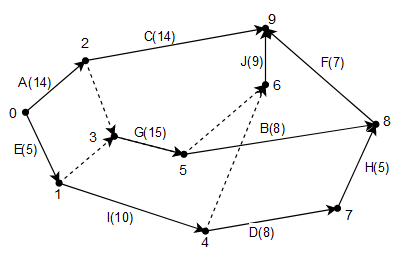
\includegraphics[width=0.7\linewidth]{./img/graf-2.PNG}
        \caption{Porządek wykonywania zadań w postaci grafu krawędziowego.}
        \label{fig:graf-2}
    \end{figure}
    Rysunek ~\ref{fig:graf-2} przedstawia porządek wykonywania zadań w postaci grafu krawędziowego wraz z posortowanymi wierzchołkami.
    \item Następnie obliczam najwcześniejsze momenty rozpoczęcia:
    \begin{flalign*}
        & T_p0 = 0 &&\\
        & T_p1 = 0 + 5 = 5 &&\\
        & T_p2 = 0 + 14 = 14 &&\\
        & T_p3 = \max{(5 + 0, 14 + 0)} = 14 &&\\
        & T_p4 = 5 + 10 = 15 &&\\
        & T_p5 = 14 + 15 = 29 &&\\
        & T_p6 = \max{(15 + 0, 29 + 0)}= 29 &&\\
        & T_p7 = 15 + 8 = 23 &&\\
        & T_p8 = \max{(29 + 8, 23 + 5)} = \max{(37, 28)} = 37&&\\
        & T_p9 = \max{(5 + 14, 29 + 9, 37 + 7)} = \max{(17, 38, 44)} = 44&&\\
    \end{flalign*}
\end{enumerate}
\subsection{Harmonogram o minimalnym czasie wykonania}
\subsection{Minimalny czas realizacji przedsięwzięcia przy określonym budżecie}
\subsection{Dobór zadań przy wprowadzonym ograniczeniu NS}
\subsection{Najkrótszy czas wykonania przedsięwzięcia, gdy zadanie B nie może zakończyć się przed zakońćzeniem zadania A}
\lstlistoflistings
\listoffigures
\listoftables

\end{document}
